\chapter{Completed Formative Work: Visual Vulnerability Analysis}
\label{ch:vulnerability}

The first design study of this proposed dissertation is a 15-month remote collaboration with defense analysts at the U.S. Army Research Laboratory. They were were trying to improve the safety of military vehicles using ballistic simulations to understand how vehicles may be vulnerable. Based on their findings, they would recommend changes to vehicle design. We worked with three analysts to understand how they used ballistic simulation results and we created a visualization tool to support their analysis. 

%They worked with ballistic simulation data: output attributes of physics-based simulations, 3D computer aided design models, and abstract relationships between vehicle components. Analysts used insights from this data to debug simulation inputs, identify components likely to be damaged, plan live-fire testing, and ultimately make recommendations about vehicle design. 

This design study is a formative project of this proposed dissertation as we used creativity methods to understand our collaborators' needs given limited time to meet in person. The creativity methods revealed visualization needs at a high level of abstraction that we investigated in more detail using contextual inquiry. This project also provides qualitative data to support the proposed creativity workshop framework. 

In this chapter we describe the project's contributions, summarize the resulting visualization tool, reflect on our use of creativity methods, and list the project's publications.

\section{Contributions}

This design study had three primary contributions: 1) a problem characterization, data abstraction, and task analysis for the domain of vulnerability analysis; 2) ShotViewer, a validated software prototype for visual vulnerability analysis; and 3) a reflection on creativity methods that will be part of this proposed dissertation's visualization creativity workshop framework.

It also had three secondary contributions: 1) a strategy for exploiting view-design parallelism while creating multiview visualizations based on a reflection of our work; 2) four recommendations for conducting design studies in large organizations with sensitive data; and 3) an algorithm that increased the computational efficiency of the ballistic simulations.

In the next section, we briefly describe the primary contributions. Please see the publications at the end of this chapter for more details about all of the contributions. 

\section{ShotViewer: Visualizing Ballistic Simulations}

We worked with analysts who were trying to understand the results of ballistic simulation software. The simulations are best explained by looking at its origins: an optical ray tracer~\cite{Butler2007}. Ray tracers compute photon paths through an environment, shade surfaces using physically-based lighting models, and output pixel color based on primary visibility rays. Ballistic simulations replace photons with {\bf shots}, a projectile being simulated, compute energy transfer using physically-based penetration models, and simulate the shot's impact on vehicle functionality using fault trees~\cite{SURVICEEngineering2013}. Historically, the simulations output statistical summaries such as the total vulnerable area of a vehicle, but these summaries have a nebulous definition that make it almost impossible to reason about why a vehicle may be vulnerable~\cite{Guber1967}. 

The goal of this work was to create tools that visualize the rich and descriptive simulation data to supplement the numerical summary values. Through creativity methods and contextual inquiry, we discovered that analysts needed to compare the simulations of a few shots simultaneously to explain trends and outliers in their data. Comparing shots was difficult, however, as it required the analysts to mentally combine three disparate datatypes: the physically-based penetration models, the 3D vehicle geometry, and fault trees --- abstract relationships between vehicle components representing its capabilities.

We developed ShotViewer to support analysis of this multityped data. ShotViewer, shown in Figure~\ref{fig:03_shotviewer}, displays shots with three linked, multiform views. The Shotline View (Figure~\ref{fig:03_shotviewer}a) displays the outputs of penetration models using a 2D parametrization of the shots. The Geometry View (Figure~\ref{fig:03_shotviewer}b) displays the 3D context of shots along with a subset of vehicle geometry. And the System View (Figure~\ref{fig:03_shotviewer}c) displays the impact of shots on the vehicle's components. Please see the publications at the end of this chapter for detailed descriptions of these views and a case study where ShotViewer was used to reason about vehicle vulnerability.

\section{Creativity Method Reflection}

We used creativity methods to navigate the challenges of working remotely with analysts who were part of a large and highly secure organization. There were organizational challenges as we had to excite analysts' managers because they were the organization's gatekeepers~\cite{Sedlmair2012}. There were interpersonal challenges as we tried to establish rapport with analysts given limited time to meet in person. And there were the standard intellectual challenges of finding an interesting visualization problem.

At the project's start we spent one week at our collaborator's offices where we used creativity methods in three half-day meetings with analysts and managers from various parts of the organization. The methods consisted of visualization awareness presentations~\cite{Lloyd2011} followed by brainstorming~\cite{Osborn1953}. We used visualization awareness to show our collaborators the potential applications of visualization. We used brainstorming to understand what our collaborators saw as their most pressing challenges. 

We engaged our collaborators with visualization awareness presentations. For example, when we presented a system for visualizing spatial and non-spatial biomechanical data developed by Keefe et al.~\cite{Keefe2009}, our collaborators saw the potential usefulness of a linked multiview system. A manager said that he wanted a similar system to explain ballistic simulation results as he said ``\emph{[the data behind simulations] is intelligible to only a few people and making sense of it is labor intensive."} 

Brainstorming helped us to discover the labor intensive parts of this analysis. All of the analysts had slightly different workflows and goals, but they used the same simulation software. During the brainstorming, all of the analysts had ideas about how visualization could help them reason about their combined spatial and non-spatial simulation input and output. This became the focus of our design study.

We investigated their analysis in detail using contextual inquiry~\cite{Holtzblatt1993}. The analysts and their managers were engaged with the contextual inquiry due, in part, to the creativity methods. After the contextual inquiry, we ultimately built ShotViewer to support the analysis of spatial and non-spatial ballistic simulation data.

\section{Conclusion and Publications}

In this design study, we used creativity methods to understand the needs of analysts in a large and highly secure organization. We then created and validated ShotViewer, a tool for visualizing multityped ballistic simulation data. 

This is a formative project of our proposed dissertation for two reasons. First, this project demonstrates that creativity methods and traditional contextual inquiry are complementary --- creativity methods provide an overview of domain challenges while contextual inquiry provides details about specific challenges. Second, it provides qualitative data to support the proposed creativity workshop framework. 

This project resulted in two publications. These papers will form this chapter in the proposed dissertation:

\begin{itemize}
    \item design study in Computer Graphics Forum, presented at EuroVis 2015 ~\cite{Kerzner2015}
    \item graphics algorithm in the Journal of Computer Graphics Techniques~\cite{Gribble2014}
\end{itemize}


\begin{figure}
 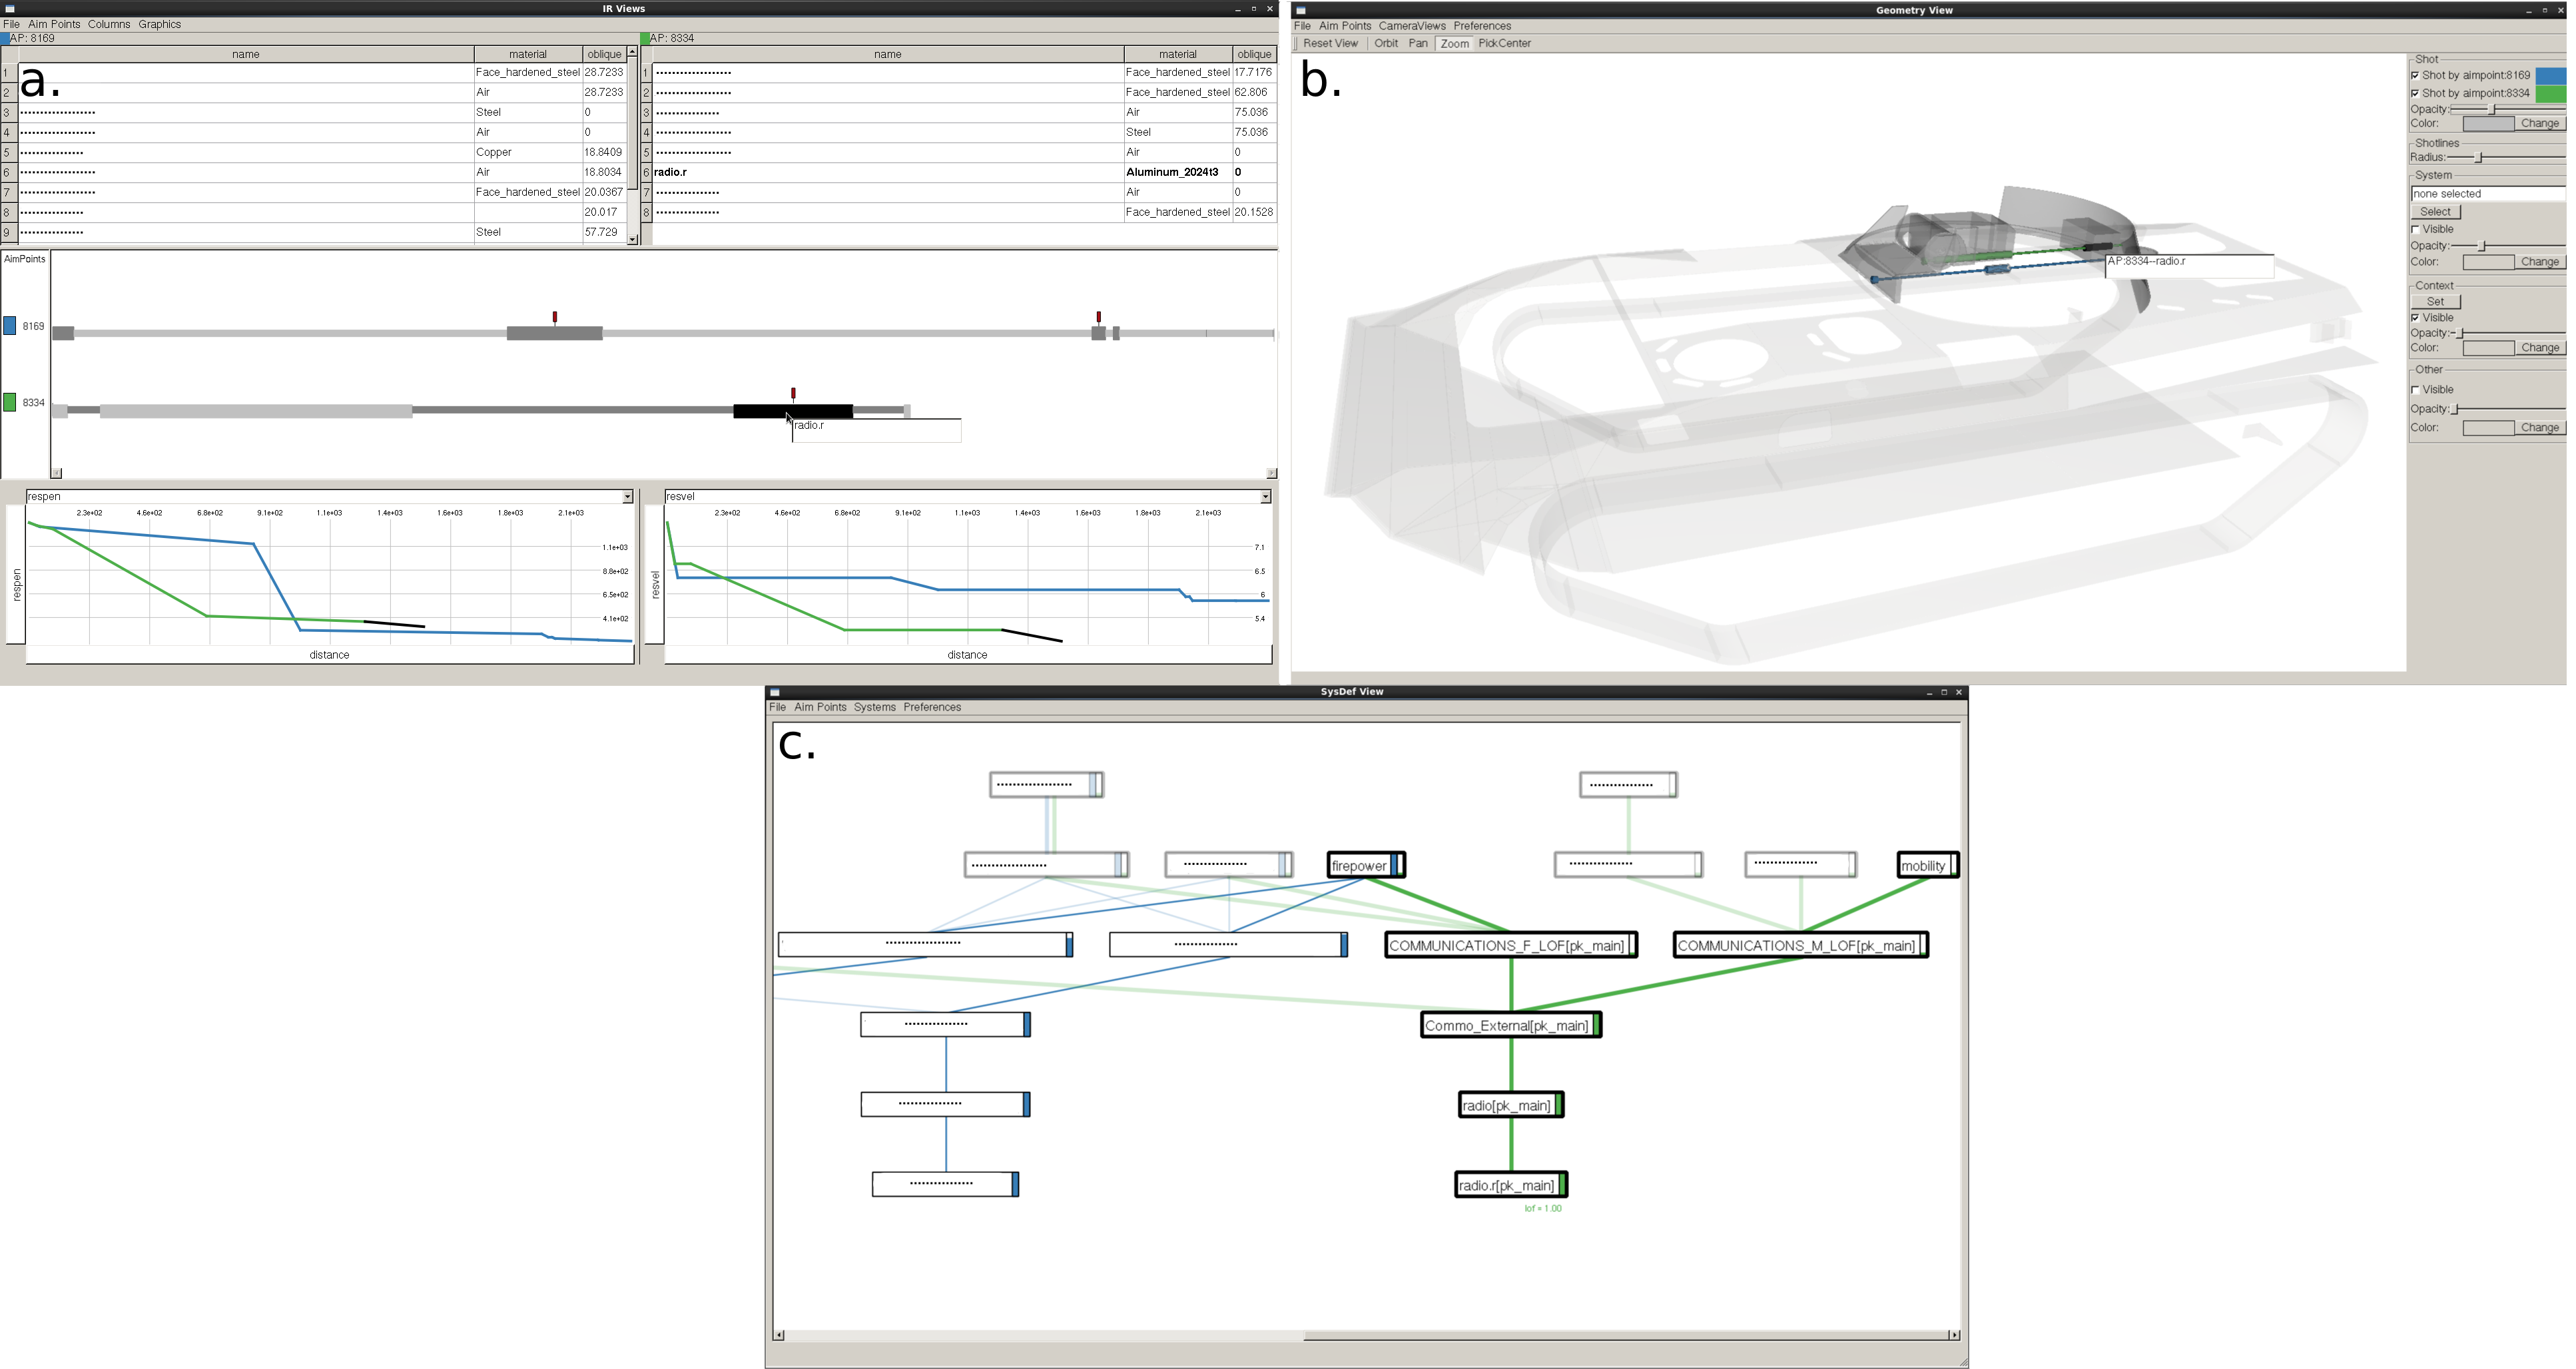
\includegraphics[width=\linewidth]{sources/figures/03_shotviewer}
  \caption{Shotviewer, software that supports visual analysis of spatial and nonspatial ballistic simulation data for vulnerability analysis. It consists of three linked views: a) the Shotline View displays an abstract representation of shots' paths through a vehicle; b) the Geometry View shows shots' 3D spatial context; and c) the System View visualizes the propagation of damage through a vehicle's systems. In this example, the green shot damages the vehicle's radio which impacts the vehicle's mobility and firepower capabilities.}
\label{fig:03_shotviewer}
\end{figure}